%The paper size, font size and document type are defined in the following
\documentclass[a4paper,12pt]{article}

%Uncomment the following line, if you write in Finnish (special characters)
%\usepackage[utf8]{inputenc}

%\usepackage[finnish]{babel}
\usepackage[english]{babel}

\usepackage{graphicx}
\usepackage[parfill]{parskip}

%useful special symbols:
\usepackage{amssymb}
\usepackage{latexsym}
\usepackage{amsmath}
\usepackage{amsthm}

\usepackage[toc,page]{appendix}

%a useful package if you write url addresses:
\usepackage{url}
\usepackage{hyperref}

%a package for figures:
% \usepackage[dvips]{color}
\usepackage{epsfig}

%a package for rotated figures and tables:
\usepackage{rotating}

\usepackage{biblatex}
\addbibresource{references.bib}

\usepackage{listings} % For including code
\usepackage{xcolor}   % For defining code colors

%% Define custom colors for the code
\definecolor{codegreen}{rgb}{0,0.6,0}
\definecolor{codegray}{rgb}{0.5,0.5,0.5}
\definecolor{codepurple}{rgb}{0.58,0,0.82}
\definecolor{backcolour}{rgb}{0.95,0.95,0.92}

% Define Python code style
\lstdefinestyle{mystyle}{
    backgroundcolor=\color{backcolour},   
    commentstyle=\color{codegreen},
    keywordstyle=\color{magenta},
    numberstyle=\tiny\color{codegray},
    stringstyle=\color{codepurple},
    basicstyle=\ttfamily\footnotesize,
    breakatwhitespace=false,         
    breaklines=true,                 
    captionpos=b,                    
    keepspaces=true,                 
    numbers=left,                    
    numbersep=5pt,                  
    showspaces=false,                
    showstringspaces=false,
    showtabs=false,                  
    tabsize=4
}

% Apply the style to Python listings
\lstset{style=mystyle}

\graphicspath{ {./figures/} }

%if you want smaller page margins, uncomment and adjust the following
%\textheight=24.3cm
%\topmargin=-1.8cm
%\textwidth=16.7cm
%\oddsidemargin=-0.3cm
%\evensidemargin=0.0cm


%Create your own environments
\newtheorem{definition}{Definition}
\newtheorem{example}{Example}
\newtheorem{theorem}{Theorem}

%and useful macrosfor faster writing (benefit: you can change the notations 
%later, e.g., two possible notations for your vector x)
\newcommand{\Mmatr}{\ensuremath{\mathbf{M}}}
\newcommand{\xvec}{\ensuremath{\overline{x}}}
\newcommand{\xvecII}{\ensuremath{\mathbf{x}}} %alternative def
\newcommand{\Xset}{\ensuremath{\mathbf{X}}}
\newcommand{\fr}{\ensuremath{\mathit{fr}}} %just neater typing

%If you want to remove the space before paragraphs uncomment the following.
%Remember then to leave an empty line between paragraphs! 
%\setlength{\parindent}{0pt}


\title{MDM-2024 Homework N}
\author{Cuong Nguyen (101559968), Petteri Raita (909635),\\and Raihan Gafur (101555441)}

%Uncomment the following, if you don't want the date to be printed
%\date{}

\begin{document}

\maketitle
\tableofcontents
\newpage

\listoffigures
\newpage

\section{Improved Algorithm}

The improved algorithm focuses on the selection of cliques based on the smallest degree nodes and uses a theorem to prune the search space efficiently.
The primary improvement lies in selecting cliques starting with nodes that have the smallest degree, \( \deg(v) \), in the entire graph.

\begin{theorem}
    \label{thm:pruning_theorem} % Label for referencing
    If
    \[
        f(S) < 1 - \frac{\deg(v) (1 - \alpha)}{(|S| - 1) \alpha}
    \]
    for any \( v \in S \), then none of \( S \)'s supersets can be an \( \alpha \)-clique.
\end{theorem}

\paragraph{Pruning Mechanism Using Theorem}
The pruning mechanism is governed by the ~\autoref{thm:pruning_theorem} that sets a condition on when a set \( S \) and its supersets can be classified as non-\( \alpha \)-cliques. For effective pruning:
\begin{itemize}
    \item The condition must hold more frequently.
    \item The upper bound on the right-hand side (RHS) of the theorem must be maximized.
\end{itemize}
Maximizing the RHS upper bound involves minimizing the negative term associated with \( \deg(v) \). Therefore, iterating over nodes from the smallest to largest degree makes the pruning happen as often as possible.

\paragraph{Illustration}
A visual representation of the improvement is shown in  ~\autoref{fig:improved_algorithm}. In the graph, the differing values tested candidates per  \(\alpha\), show the computation performance of the improved algorithm. For smaller  \(\alpha\) values, the effect is more pronounced, but even for the  \(\alpha = 0.8\) , the improved algorithm does 47 comparisons less. With  \(\alpha\) reaching 1, there is no difference with the improved and traditional algorithm. This happens, since the RHS of the theorem will become always 1. The exact values of \(\alpha\) are show in ~\autoref{tab:tested_candidates}

\begin{table}[h]
    \centering
    \begin{tabular}{ccc}
        \hline
        \(\alpha\) & Basic Algorithm & Improved Algorithm \\
        \hline
        0.5        & 1613            & 1471               \\
        0.6        & 1261            & 1127               \\
        0.7        & 1006            & 902                \\
        0.8        & 621             & 574                \\
        \hline
    \end{tabular}
    \caption{Exact values of tested candidates per  \(\alpha\)}
    \label{tab:tested_candidates} % Added label for referencing
\end{table}


\paragraph{Impact of Graph Size on \(\alpha\)}
For future research, the effect of the size of the graph for pruning could be studied. The size might affect the number of candidates tested that the pruning affects. Possbily in larger graphs, the impact of the improved pruning algorithm might save more tested candidates.

\begin{figure}[h]
    \centering
    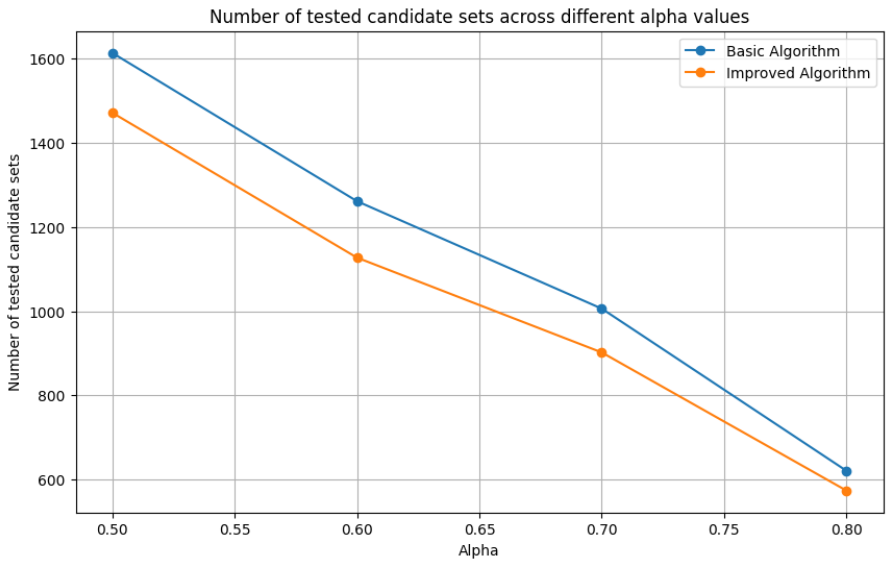
\includegraphics[width=0.8\textwidth]
    {figures/improved_algorithm.png}
    \caption{Number of tested candidates per \(\alpha\)}
    \label{fig:improved_algorithm}
\end{figure}

% include tex files of sections here, e.g.
% \input{section1.tex}
% \input{section2.tex}

%Bibliography style. The alpha style generates references with 
%first letters and year. If you prefer numbers, use style plain.
% \bibliographystyle{alpha}
% \bibliographystyle{plain}
% \bibliography{ref}

% \printbibliography{}

% Demo for adding appendices
% \begin{appendices}
%     All code is publicly available on GitHub at \url{https://github.com/ancuongnguyen07/CS-E4650/tree/master/hw5}
% \end{appendices}


\end{document}
